\section{Question 1}
\subsection{Part A}
The number of hidden units primarily affects the speed that the model converges at.  Looking at the figure below, 20 hidden units appears to be the best number.  However, by the third epoch, 5 hidden units has similar performance and by the ninth epoch, 100 hidden units has converged.  This is likely because the function to classify the outputs is relatively simple.  For a more complex problem, the number of hidden units would also affect the accuracy of the classifier.  However, having too many hidden units can allow the model to overfit.  This can be more clearly seen in Part B.
\begin{figure}[H]
	\centering
	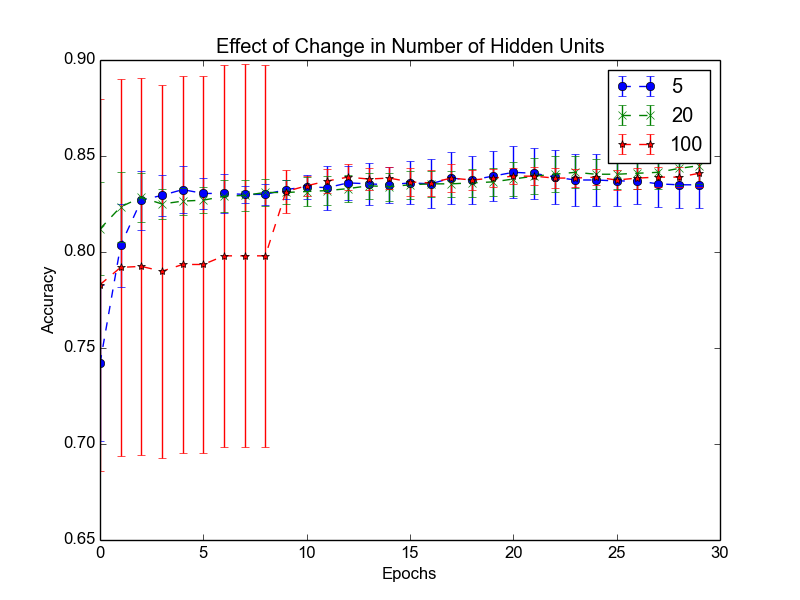
\includegraphics[width=0.6\textwidth]{../train1/hidden_units.png}
	\caption{Effect of changing number of hidden units}
\end{figure}

\subsection{Part B}
The biggest effect that training time has is that as training time increases, performance begins to degrade.  The model is overfitting to the training set which is making it less generalizable.  As a result, performance degrades on the test set.  In an extreme case, too little training time will cause the model not to achieve maximum performance, but for this data set, that is less than 5 epochs.  The results of short training time can be seen in Part A.
\begin{figure}[H]
	\centering
	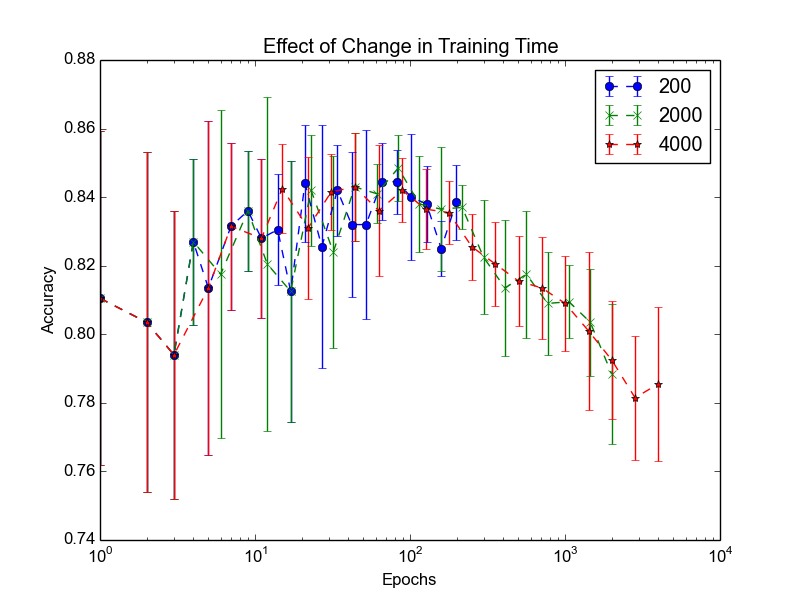
\includegraphics[width=0.6\textwidth]{../train1/epochs.png}
	\caption{Effect of changing traning time}
\end{figure}

\subsection{Part C}
The size of the learning rate affects how quickly the classifier converges.  With very small steps, the classifier takes a long time to converge.  With very large steps, the classifier diverges and always performs poorly.  An appropriate step size allows for convergence to happen in a reasonable amount of time.
\begin{figure}[h]
	\centering
	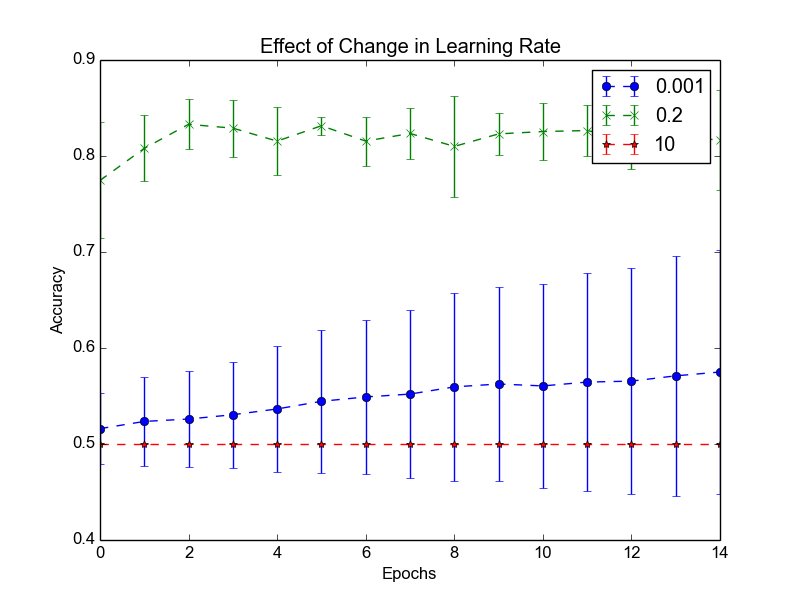
\includegraphics[width=0.6\textwidth]{../train1/learning_rate.png}
	\caption{Effect of changing learning rate}
\end{figure}

\subsection{Part D}
I found an interesting bug (feature?) in Python when using multiprocessing.  The cause (I think) is that because the processes spawn so quickly, they all use the same machine time to generate their random weight initializations.  This results in all of the newtorks having the same results.  This is even more surprising since the data is shuffled for every epoch.  I believe that again the shuffling was happening the same for all of the trials.  I was eventually able to cause the weights to be different by seeding the generator with different values for each trial.  An intersting problem that only occurs when using multiprocessing.

Some other parameters that the can change convergence time and network performance are the initialization weights of the network and shuffling the data during processing.  I examined how initialization of the weights affects the algorithm.  The legend shows the magnitude of the initial values.  For very small magnitudes of initial weights, the network does not change much over the course of training.  It always predicts the same value which results in 50\% accuracy because of the distribution of the testing set.  For very large values, numerical saturation occurs and the network begins to output NaNs which are always classified as incorrect.  This results in 0\% success.  
\begin{figure}[h]
	\centering
	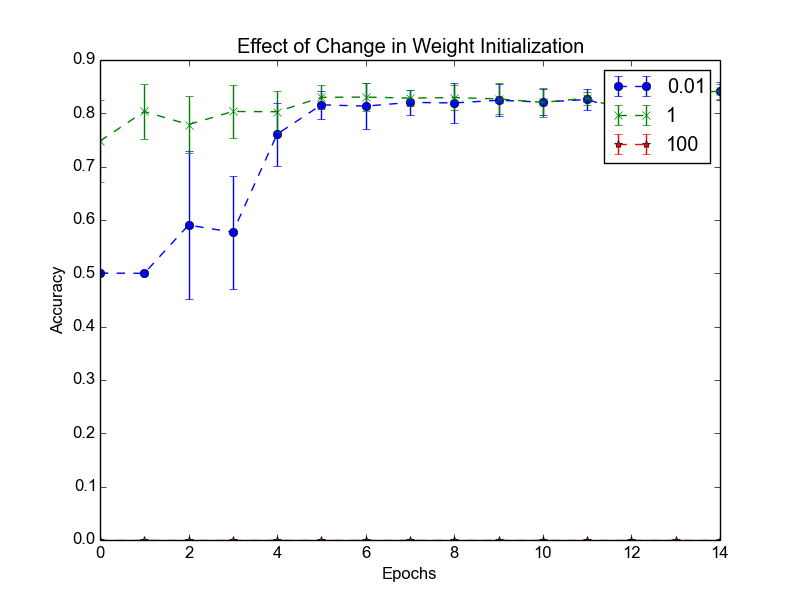
\includegraphics[width=0.6\textwidth]{../train1/weights.png}
	\caption{Effect of classifier on different test data sets}
\end{figure}


\subsection{Part E}
Different data sets have similar performance.  Performance on dataset two appears to be the best.  Test set 2 has the closest distribution of passes and fails as the model.  Although, this does not completely explain the difference.  The biggest issue is likely that the training data sets differs the least from set 2.  Set 1 has many more passes than fails.  This might suggest that the model tends to predict more passes than fails (false positives).  Since Set 3 has more fails than passes, this bias may also explain the poorer performance of the classifier on the third data set.
\begin{figure}[h]
	\centering
	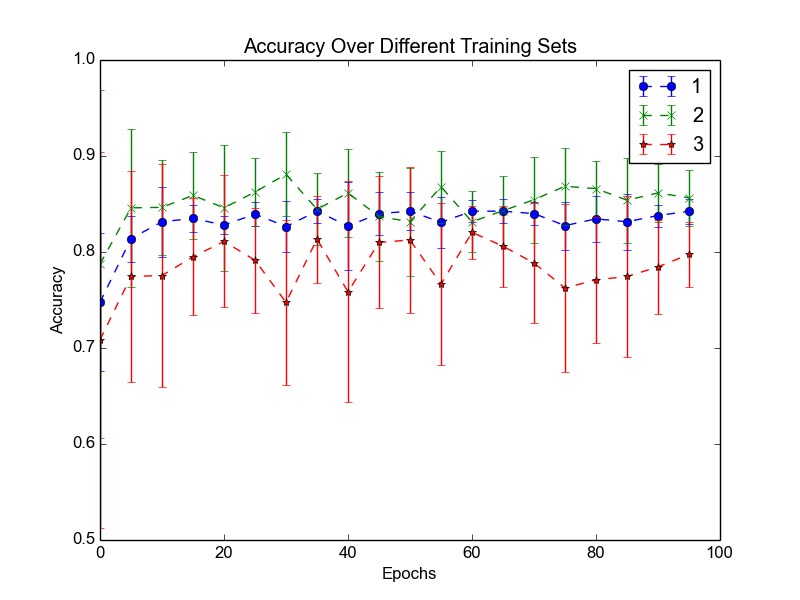
\includegraphics[width=0.6\textwidth]{../train1/data_sets.png}
	\caption{Effect of classifier on different test data sets}
\end{figure}